%%%%%%%%%%%%%%%%%%%%%%%%%%%%%%%%%%%%%%%%%%%%%%%%%%%%%%%%%%%%%%%%%%%%%%%%%%%%%%%%
%2345678901234567890123456789012345678901234567890123456789012345678901234567890
%        1         2         3         4         5         6         7         8
% THESIS Chapter

\chapter{Previous required knowledge}
\label{chap:first}
\ifpdf
    \graphicspath{{Chapter1/Figures/PNG/}{Chapter1/Figures/PDF/}{Chapter1/Figures/}}
\else
    \graphicspath{{Chapter1/Figures/EPS/}{Chapter1/Figures/}}
\fi


\section{LPWAN}
\label{sec:f-lpwan}
LoRa and LoRaWAN protocols are based on the LPWAN technology.
LPWAN stands for “Low Power Wide Area Network” and it allows radio-
equipped devices to communicate more efficiently and over longer
distances. This emergent technology had the goal of finding a better
data transmission protocol than other technologies such as Bluetooth,
Wi-Fi or 3G/4G. The low-power consumption and the long range
transmission that this technology offers, positions it as a cost-effective
solution when compared with the other big technologies. As LPWAN is
not concerned with transmitting big quantities of data, it offers aspects
that simply others can't complete such as the coverage of long distances
as it can be appreciated in the figure below.
\begin{figure}[htbp]
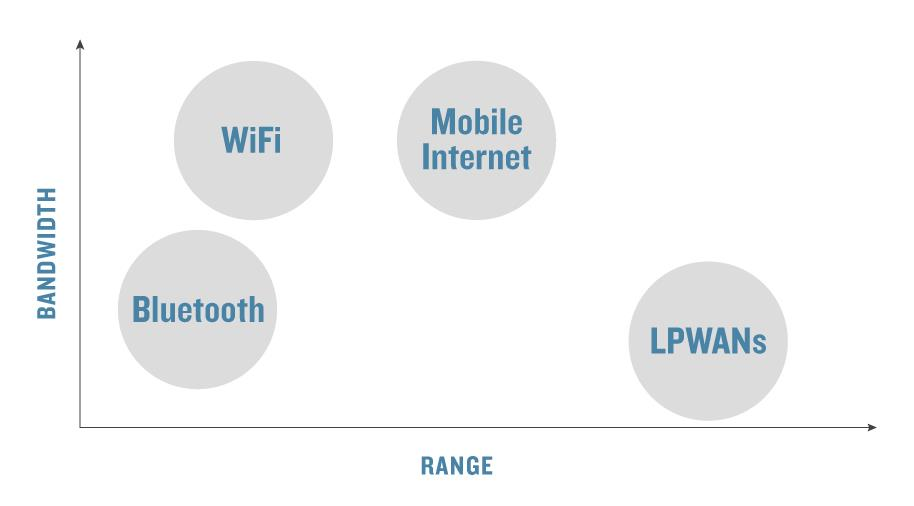
\includegraphics[width=\linewidth]{rangevsband.png}
\caption{Graph comparison of range and bandwidth for different data transmission technologies.}
\end{figure}

This is why LPWAN has become one of the fastest growing spaces in
the Internet of Things (IoT) ecosystem. One of the biggest and most
interesting applications of this data transmission technology is on the
Smart Cities field. This protocols are a perfect solution for the Smart City
data networks, which requires low data rate but constant data streams
and the coverage of long distances with the benefit of using significantly
less power than other data network platforms. Shanghai is a perfect
example of a Smart City where LPWAN is used in order to connect
thousands of sensors to measure the air quality and human movement, more info 
\href{https://www.citiesforum.org/news/what-made-shanghai-the-worlds-no-1-smart-city}{here}.
The future of this technology is bright as IoT devices are growing a 12\%
annually according to a \href{https://cdn.ihs.com/www/pdf/IoT_ebook.pdf}{IHS Markit report}.
and LPWAN is one of the greatest spaces in the IoT ecosystem. LoRa and LoRaWAN are
realizations of the Low Power WAN concept, and with such high demand
for the technology both are having great impulse in their development.
\section{LoRa}
\label{sec:f-lora}
LoRa is the protocol which defines the physical (radio) layer of the
communications in TTN. This protocol fixes the
frequency band and defines the modulation that is used to transmit data
which enables the long-range communication link.\\
The frequency band depends on the region in which you are, for
example, in the US they use a band from 902.3 to 914.9 MHz, here in
Europe the band goes from 863 to 870 MHz as it's ilustrated on the next table:\\

\begin{table}[htbp]
\centering
\setlength{\arrayrulewidth}{0.5mm}
\setlength{\tabcolsep}{18pt}
\renewcommand{\arraystretch}{2}
\begin{tabular}{ |p{5cm}|p{5cm}| }
\hline
\multicolumn{2}{|c|}{\cellcolor[HTML]{85C1E9}Frequency band depending on the region } \\
\hline
\cellcolor[HTML]{AED6F1} Region & \cellcolor[HTML]{AED6F1} Frequency (Mhz) \\
\hline
Asia & 433  \\
Europe & 863-870 \\
US & 902-928 \\
Australia & 915-918  \\
Canada & 779-787  \\
China & 470-510  \\
\hline
\end{tabular}
\caption{frequency band of different regions}
\end{table}

The LoRa modulation is based on the Spread Spectrum technique and
it's crucial for the long distance communication. This technique spreads
the signal all over the frequency band and it allows LoRa to be very
robust to interferences and noise, allowing the signal to reach longer
distances. More precisely it's called chirp modulation and it transmits
symbols encoding them into multiple signals of increasing (upchirp) or
decreasing (downchirp) radio frequencies. A LoRa transmission always
starts with 8 upchirps and 2 downchirps as we can see in the figure
number 1.2.
\begin{figure}[htbp]
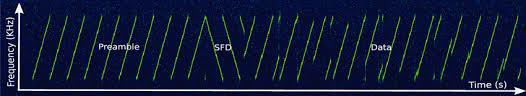
\includegraphics[width=\linewidth]{lorainitchirp.png}
\caption{Snapshot of a LoRa transmission}
\end{figure}
In LoRa communications we are able to reduce our data rate in order to
gain range by changing the Spreading Factor. The Spreading Factor
means the number of raw bits that can be encoded in a symbol.
(“Modelling and Performance Evaluation of LoRa Network Based on
Capture ...”) The SF value goes from 7 to 12 and as we increase this
value the number of raw bits in a symbol increase and this leads to a
gain of range but also to a reduction of data rate, to an incrementation
of the time on air and to more battery consumption. \\
The SF value can vary from 7 to 12 both included, trading data rate with
range. The increase or decrease in data rate is proportional to the time
on air, greater meaning not only more battery consumed but also greater
chance of collision. The increase in range is due to the higher sensitivity
of the receiver at greater values of SF. In short, increasing a level the
SF means stretching the signal twofold, with its corresponding higher
power consumption but better range.\\
LoRa has to deal with the specific regulations and norms of each region.
Here in Europe we must comply the following rules:
\begin{itemize}
   \item For uplink, the maximum transmitted power is limited to 25 mW
(14dBm) 
    \item For downlink, the maximum transmission power is limited to 0.5W
(27dBm)
    \item There is between an 0.1\% and 1\% duty cycle per day. This means
            that the time on air of the transmission must not exceed a
            proportion of the total time.
    \item Maximum allowed antenna gain +2.15 dBi
\end{itemize}
\section{TTN and LoRaWAN}
\label{sec:f-ttnandlora}
LoRaWAN defines the communication protocol and the system
architecture, it acts like a MAC layer for LoRa packets. The Things
Network is a LoRaWAN network operator that use this protocol and its
network topology to give free LoRaWAN connectivity. \\
The LoRaWAN network topology, as it's represented in figure 1.3,
consist of 4 layers: end-nodes, gateway, network server and application
server.
\begin{figure}[htbp]
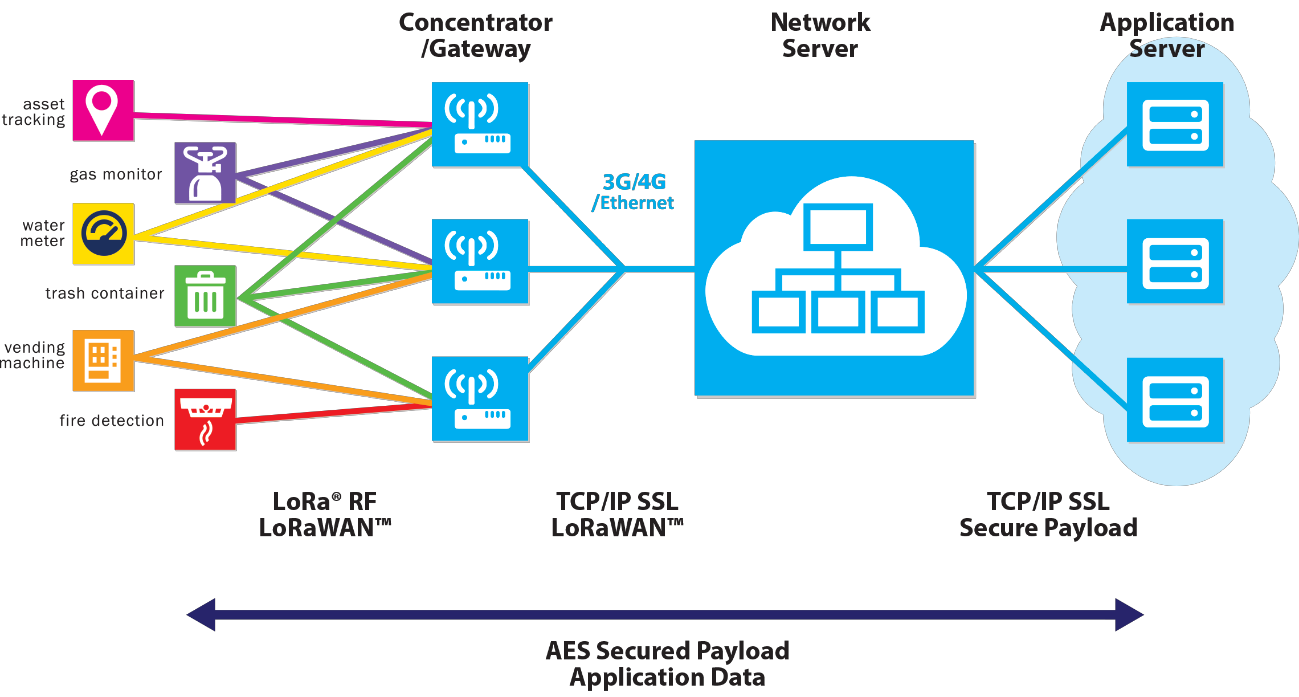
\includegraphics[width=\linewidth]{ttnarch.png}
\caption{LoRaWAN network topology}
\end{figure}
Gateways are able to listen from hundreds of end nodes at the same
time, even if those nodes are transmitting at different frequencies or SF.
The data transmitted through the gateways arrives to the network server
via TCP/IP. Then the network server (NS) sends those packets to the
application server (AS) and if it is needed, a different server called join
server (JS), enters in the process. This server stores the sensitive parts
of LoRaWAN applications such as the root keys and generates the
session keys when a join procedure takes place.\\
In LoRaWAN communications we distinguish two types of transmissions
depending on the sense of communication. An uplink message is sent
from an end-node to a network server and in the case of a downlink
message the message in sent from a network server to a specific device.

\begin{itemize}
    \item \textbf{Uplink message:} this message uses the 
    LoRa radio packet explicit mode, which consists of a physical 
    header (PHDR) and a cyclic redundancy check (CRC) header (PHDR-CRC). 
    Another CRC is required to protect the integrity of the payload; all of
    them are together inserted by the radio transciver in the following way:
    \begin{center}
    \begin{tabular}{ |c|c|c|c|c| } 
     \hline
     Preamble & PHDR & PHDR-CRC & PHYPayload & CRC\\ 
     \hline
    \end{tabular}
    \captionof{table}{Uplink message format.}
    \end{center}
    
    \item \textbf{Downlink message:} The structure is very similar to the uplink message, the only difference is that in a downlink message there is no existence of CRC:
    \begin{center}
    \begin{tabular}{ |c|c|c|c| } 
     \hline
     Preamble & PHDR & PHDR-CRC & PHYPayload \\ 
     \hline
    \end{tabular}
    \captionof{table}{Downlink message format.}
    \end{center}
\end{itemize}
    
This PHYPayload that both, the uplink and the downlink messages contains, starts with a single-octet MAC header (MHDR), followed by a MAC payload (MACPayload) and finishing with a 4-octet message
integrity code (MIC):
\begin{center}
\begin{tabular}{ |c|c|c| } 
    \hline
    MHDR & MACPayload & MIC \\ 
    \hline
\end{tabular}
\captionof{table}{PHYPayload}
\end{center}

The MHDR defines the type of the message that is sent. Those types are join request, join accept, unconfirmed data up/down and confirmed data up/down, where confirmed means that it has to be acknowledged by the receiver, while unconfirmed does not require that.

The MACPayload contains a frame header (FHDR), which is the device address of an end-device (DevAddr), followed by an optional port field (FPort) and an optional frame payload field (FRMPayload):

\begin{center}
\begin{tabular}{ |c|c|c| } 
    \hline
    FHDR (DevAdd) & FPort & FRMPayload \\ 
    \hline
\end{tabular}
\captionof{table}{MACPayload}
\end{center}

Three device classes are defined in LoRaWAN:
\begin{itemize}
    \item Class A: in this class after the uplink transmission two reception
windows are set in order to receive downlink messages. A stands
for All, since all devices must implement this functionality.
    \item Class B: in addition to class A devices, this class open extra
receive windows at scheduled times. Time synchronized beacons
are sent from the gateway to fix those scheduled times in the end
node.
    \item Class C: this type of devices have almost all time open receive
windows and are only closed when transmitting.
\end{itemize}
Class A is the most common class as it is the most energy efficient.\\
The frequency band defined by LoRa is divided into 8 channels. In the
case of downlink messages there are 8 channels used by the first
reception window and another one used by the second window. Due to
the regulations in Europe each channel must be of 125 KHz of
bandwidth. During a data transmission the channel is constantly
changing in order to make the communication more robust to
interferences.\\
An important mechanism that is used to control the uplink connection
between the end node and the gateway is the Adaptative Data Rate
(ADR). This protocol is able to modify automatically parameters like the
Spreading Factor or the transmission power according to the signal
power that the gateway is receiving. As it's explained before, the SF also
affects the power used by the node so this mechanism is able to find the
optimal point in which the node is only using the necessary power. The
Things Network allows to disable or enable it depending on your
purpose. If the device is stationary, TTN recommends to leave the ADR
active, but if the end node is supposed to move, the SF and power
should be in charge of the programmer.\\
The ADR algorithm is simple, but has important ramifications on 
the performance if the device is not stationary.
The reason for this is that the ADR algorithm was designed in order
to provide the best bandwidth utilization and the best battery life
to devices with an stable radio communication. From this falls that 
a moving end node is not the optimal target for the algorithm. Nevertheless, 
the effects of it are easy enough to analize. 
Currently The Things Stack takes the 20 most recent uplinks, 
starting at the moment the ADR bit is set. 

For any LPWAN technology it's crucial to incorporate security.
LoRaWAN uses two layers of security: one for the network layer and
another one for the application layer. The network security layer ensure
the authentication and all the transmission is encrypted by the
application layer with the AES method. Private session keys are needed
and there are two main different methods to obtain them:
\begin{itemize}
    \item[-] {\bfseries Over the air activation (OTAA):} in this method the device needs
to be equipped with a DevEUI that identifies the device, with a
AppEUI to identify the application and with a AppKey that is used
to sign an initial join request. Once the initial request is validated,
the join server generates the two session keys, and they are send
to the end node. Those keys are the NwSKey and the AppSKey
and are used to identify the network server and to encrypt the
payload.
    \item[-] {\bfseries Activation by personalization (ABP):} with this method you can
access the network without a join request because the device is
already equipped with the AppSKey and the NwSKey.
\end{itemize}
Usually the OTAA method is preferred, this is because it can generate
new session keys for each session and it allows re-key. ABP is not as
flexible as OTAA as the session keys are fixed in the device.
% add more sections and subsection here
% \subsection{Subsection One name}
% \label{sec:subsec11}
